\documentclass[french]{article}
\usepackage[T1]{fontenc}
\usepackage{fullpage}
\usepackage{babel}
\usepackage{hyperref}
\usepackage{graphicx}
\usepackage[justification=centering]{caption}
\usepackage{amsmath}
\usepackage{amssymb}
\usepackage{listings}
\usepackage{xcolor}
\usepackage{parskip}
\usepackage{enumitem}
\setlist{nosep}

\lstset{
    inputencoding = utf8,  % Input encoding
    extendedchars = true,  % Extended ASCII
    literate      =        % Support additional characters
      {á}{{\'a}}1  {é}{{\'e}}1  {í}{{\'i}}1 {ó}{{\'o}}1  {ú}{{\'u}}1
      {Á}{{\'A}}1  {É}{{\'E}}1  {Í}{{\'I}}1 {Ó}{{\'O}}1  {Ú}{{\'U}}1
      {à}{{\`a}}1  {è}{{\`e}}1  {ì}{{\`i}}1 {ò}{{\`o}}1  {ù}{{\`u}}1
      {À}{{\`A}}1  {È}{{\`E}}1  {Ì}{{\`I}}1 {Ò}{{\`O}}1  {Ù}{{\`U}}1
      {ä}{{\"a}}1  {ë}{{\"e}}1  {ï}{{\"i}}1 {ö}{{\"o}}1  {ü}{{\"u}}1
      {Ä}{{\"A}}1  {Ë}{{\"E}}1  {Ï}{{\"I}}1 {Ö}{{\"O}}1  {Ü}{{\"U}}1
      {â}{{\^a}}1  {ê}{{\^e}}1  {î}{{\^i}}1 {ô}{{\^o}}1  {û}{{\^u}}1
      {Â}{{\^A}}1  {Ê}{{\^E}}1  {Î}{{\^I}}1 {Ô}{{\^O}}1  {Û}{{\^U}}1
      {œ}{{\oe}}1  {Œ}{{\OE}}1  {æ}{{\ae}}1 {Æ}{{\AE}}1  {ß}{{\ss}}1
      {ẞ}{{\SS}}1  {ç}{{\c{c}}}1 {Ç}{{\c{C}}}1 {ø}{{\o}}1  {Ø}{{\O}}1
      {å}{{\aa}}1  {Å}{{\AA}}1  {ã}{{\~a}}1  {õ}{{\~o}}1 {Ã}{{\~A}}1
      {Õ}{{\~O}}1  {ñ}{{\~n}}1  {Ñ}{{\~N}}1  {¿}{{?`}}1  {¡}{{!`}}1
      {°}{{\textdegree}}1 {º}{{\textordmasculine}}1 {ª}{{\textordfeminine}}1
      {£}{{\pounds}}1  {©}{{\copyright}}1  {®}{{\textregistered}}1
      {«}{{\guillemotleft}}1  {»}{{\guillemotright}}1  {Ð}{{\DH}}1  {ð}{{\dh}}1
      {Ý}{{\'Y}}1    {ý}{{\'y}}1    {Þ}{{\TH}}1    {þ}{{\th}}1    {Ă}{{\u{A}}}1
      {ă}{{\u{a}}}1  {Ą}{{\k{A}}}1  {ą}{{\k{a}}}1  {Ć}{{\'C}}1    {ć}{{\'c}}1
      {Č}{{\v{C}}}1  {č}{{\v{c}}}1  {Ď}{{\v{D}}}1  {ď}{{\v{d}}}1  {Đ}{{\DJ}}1
      {đ}{{\dj}}1    {Ė}{{\.{E}}}1  {ė}{{\.{e}}}1  {Ę}{{\k{E}}}1  {ę}{{\k{e}}}1
      {Ě}{{\v{E}}}1  {ě}{{\v{e}}}1  {Ğ}{{\u{G}}}1  {ğ}{{\u{g}}}1  {Ĩ}{{\~I}}1
      {ĩ}{{\~\i}}1   {Į}{{\k{I}}}1  {į}{{\k{i}}}1  {İ}{{\.{I}}}1  {ı}{{\i}}1
      {Ĺ}{{\'L}}1    {ĺ}{{\'l}}1    {Ľ}{{\v{L}}}1  {ľ}{{\v{l}}}1  {Ł}{{\L{}}}1
      {ł}{{\l{}}}1   {Ń}{{\'N}}1    {ń}{{\'n}}1    {Ň}{{\v{N}}}1  {ň}{{\v{n}}}1
      {Ő}{{\H{O}}}1  {ő}{{\H{o}}}1  {Ŕ}{{\'{R}}}1  {ŕ}{{\'{r}}}1  {Ř}{{\v{R}}}1
      {ř}{{\v{r}}}1  {Ś}{{\'S}}1    {ś}{{\'s}}1    {Ş}{{\c{S}}}1  {ş}{{\c{s}}}1
      {Š}{{\v{S}}}1  {š}{{\v{s}}}1  {Ť}{{\v{T}}}1  {ť}{{\v{t}}}1  {Ũ}{{\~U}}1
      {ũ}{{\~u}}1    {Ū}{{\={U}}}1  {ū}{{\={u}}}1  {Ů}{{\r{U}}}1  {ů}{{\r{u}}}1
      {Ű}{{\H{U}}}1  {ű}{{\H{u}}}1  {Ų}{{\k{U}}}1  {ų}{{\k{u}}}1  {Ź}{{\'Z}}1
      {ź}{{\'z}}1    {Ż}{{\.Z}}1    {ż}{{\.z}}1    {Ž}{{\v{Z}}}1
      % ¿ and ¡ are not correctly displayed if inconsolata font is used
      % together with the lstlisting environment. Consider typing code in
      % external files and using \lstinputlisting to display them instead.      
  }



\definecolor{codegreen}{rgb}{0,0.6,0}
\definecolor{codegray}{rgb}{0.5,0.5,0.5}
\definecolor{codepurple}{rgb}{0.58,0,0.82}
\definecolor{backcolour}{rgb}{0.95,0.95,0.92}

\lstdefinestyle{mystyle}{
    backgroundcolor=\color{backcolour},   
    commentstyle=\color{codegreen},
    keywordstyle=\color{magenta},
    numberstyle=\tiny\color{codegray},
    stringstyle=\color{codepurple},
    basicstyle=\ttfamily\footnotesize,
    breakatwhitespace=false,         
    breaklines=true,                 
    captionpos=b,                    
    keepspaces=true,                 
    numbers=left,                    
    numbersep=5pt,                  
    showspaces=false,                
    showstringspaces=false,
    showtabs=false,                  
    tabsize=2
}

\lstset{style=mystyle}
\setlength{\parindent}{0pt}

\hypersetup{
  colorlinks=true,
  linkcolor=black,
  urlcolor=blue
}

\graphicspath{ {./img/} }
\title{%
    \huge IArgus  \\
    \bigskip
    \large E3 - Mise en situation \\ 
    Développeur en Intelligence Artificielle,
    titre professionnel enregistré au RNCP - École IA Microsoft by Simplon
    \vfill
    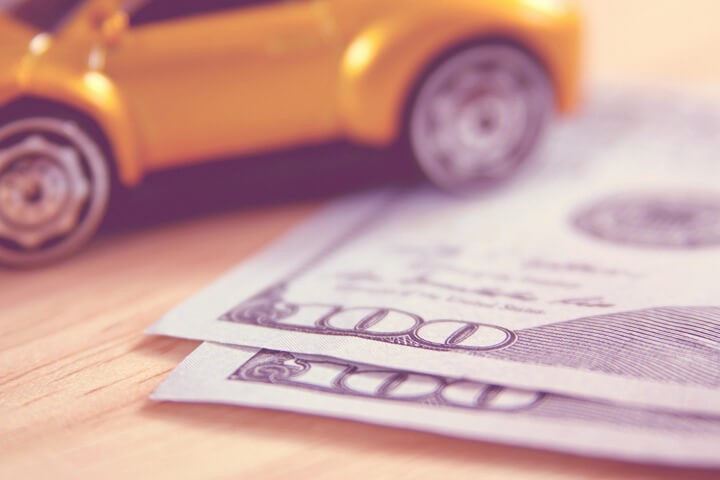
\includegraphics[width=14cm]{selling-your-old-car.jpg}
    \vfill}
\date{23 mars 2024}
\author{par Vincent Papelard}

\begin{document}
    \renewcommand{\contentsname}{Table des Matières}
    \renewcommand{\refname}{Références}
    \maketitle
    \pagenumbering{arabic}
    \pagenumbering{gobble}
    \newpage
    \tableofcontents
    \newpage
    \pagenumbering{arabic}

    \section*{Introduction}
    Depuis bientôt un siècle, l'Argus est le magazine de référence pour estimer la valeur d'un véhicule d'occasion. Fort de son statut en France, l'hebdomadaire a décidé de s'attaquer au marché américain en lançant son nouveau service, IArgus, aux États-Unis. Ce service en ligne proposera une IA qui estimera automatiquement le juste prix d'un véhicule en se basant sur des caractéristiques comme son modèle, son année de vente, son kilométrage...
    La direction de l'Argus a fait appel à nous pour développer ce nouveau service et le leur livrer avec toute la documentation nécessaire à sa mise en place, puis intégrer ce modèle à l'application IArgus qu'ils ont créée.

    La totalité du code relatif à ce dossier est disponible sur \href{https://github.com/vinpap/iargus}{GitHub}.
    \section{Contexte}
    \subsection{L'application de départ}
    Dans l'optique d'accueillir ce nouveau service, les développeurs web embauchés par l'Argus ont créé un site web qui comporte un formulaire permettant aux utilisateurs d'entrer les caractéristiques d'une voiture. C'est là que nous intervenons : nos clients de l'Argus souhaitent que la validation de ce formulaire envoie une requête à une intelligence artificielle qui estimera le meilleur prix de vente pour la voiture de l'utilisateur.
    \begin{figure}[h!]
        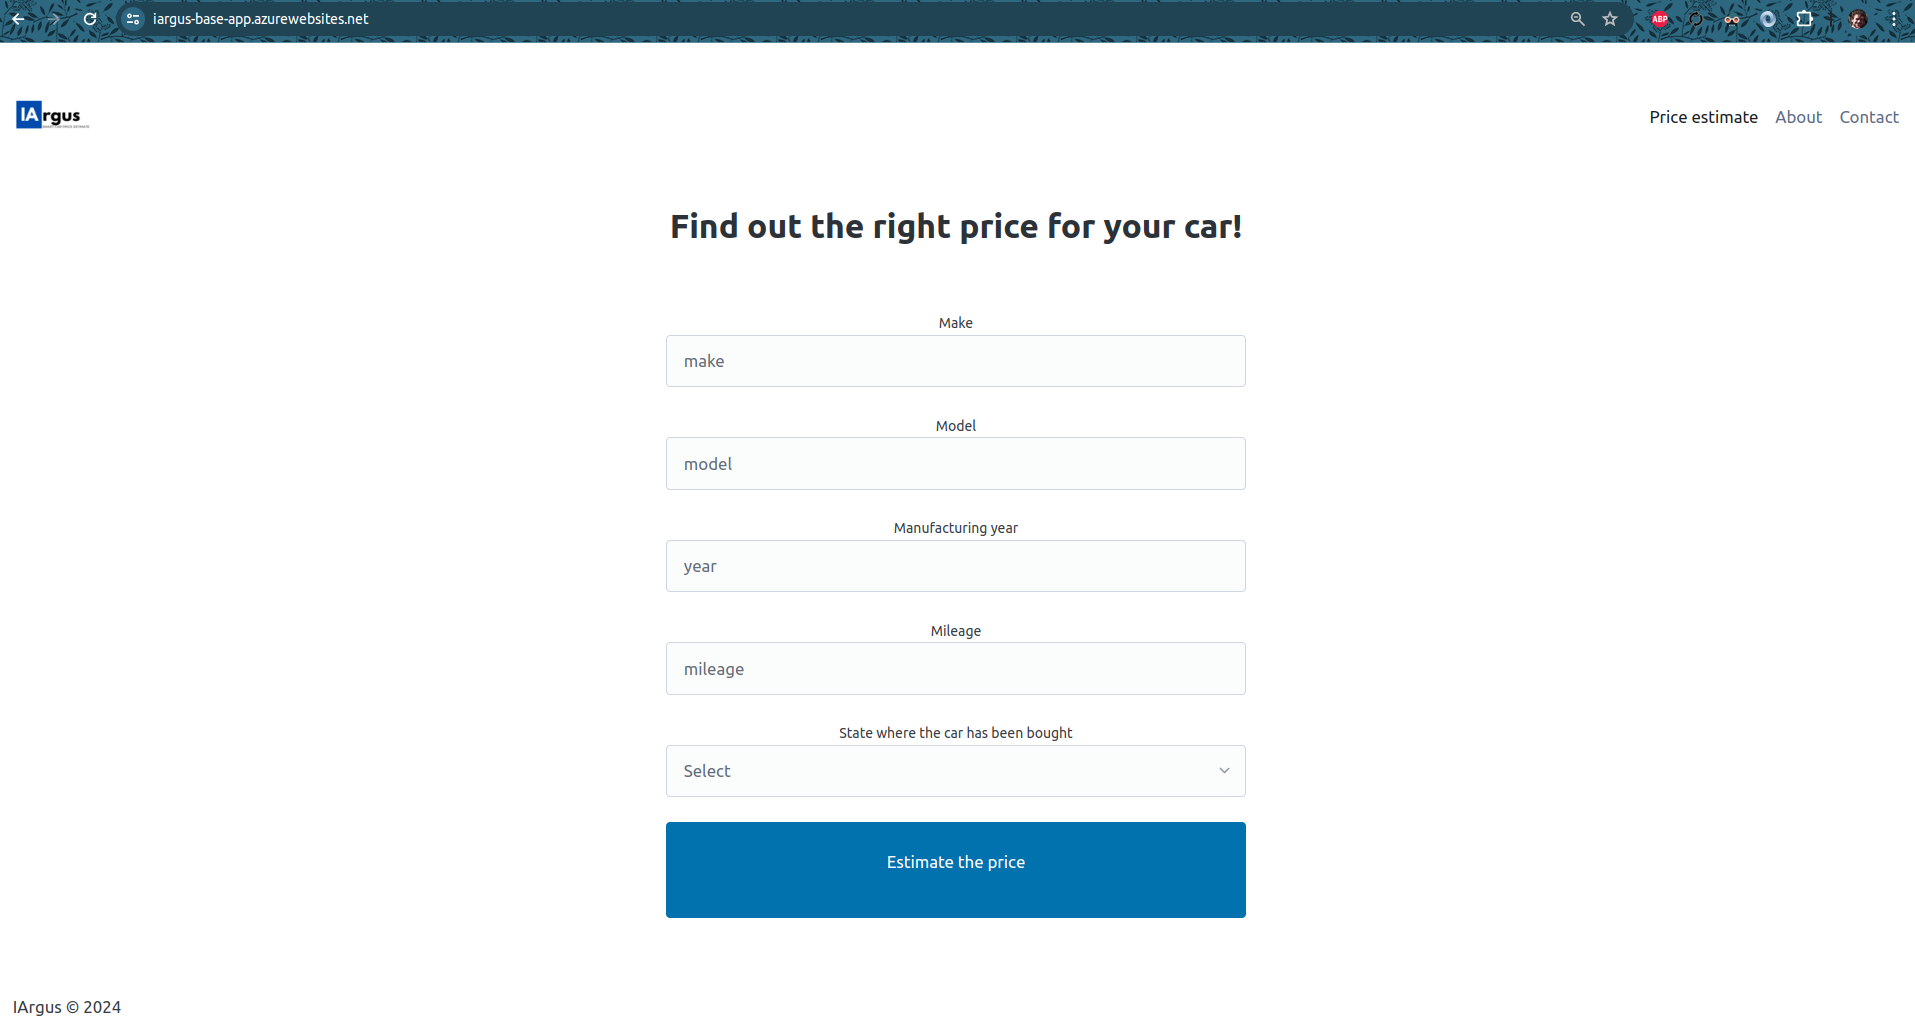
\includegraphics[width=12cm]{base_app}
        \centering
        \caption{Disponible sur la page d'accueil du site, ce formulaire permet à l'utilisateur d'entrer les caractéristiques de sa voiture pour obtenir une estimation de son prix.}
        \centering
    \end{figure}

    Cette application est déployée et disponible sur Microsoft Azure à cette adresse : \href{https://iargus-base-app.azurewebsites.net/}{https://iargus-base-app.azurewebsites.net/}.

    \subsection{Les données disponibles}
    Pour nous permettre de mener notre mission à bien, l'Argus met à notre disposition un jeu de données qui recense plus de 800 000 ventes de voitures d'occasion. Pour chaque transaction sont indiqués :
    \begin{itemize}
        \item le prix de vente, en dollars américains
        \item l'année de production de la voiture
        \item le nombre de kilomètres qu'elle a parcourus
        \item la ville où s'est déroulée la vente
        \item l'état américain où la vente a eu lieu
        \item le VIN, un identifiant unique pour chaque voiture
        \item la marque de la voiture
        \item son modèle.
    \end{itemize}
    \textbf{Remarque} : le jeu de données présenté ci-dessus est disponible \href{https://www.kaggle.com/datasets/harikrishnareddyb/used-car-price-predictions/data}{ici}.
    
    Par ailleurs, le client nous fait savoir qu'il reçoit chaque mois de nouvelles données de transactions similaires, qu'il stocke dans une base de données MySQL. Ces données pourront être utilisées pour améliorer le modèle et vérifier qu'il reste performant.
    \subsection{Exigences du client}
    Le client a quelques exigences très spécifiques en ce qui concerne le service d'intelligence artificielle dont il a besoin. Celles-ci sont les suivantes :
    \begin{itemize}
        \item l'équipe informatique d'IArgus doit disposer d'un moyen qui leur permette de visualiser simplement les performances de l'intelligence artificielle, afin de s'apercevoir rapidement de tout problème
        \item Les estimations de prix d'IArgus doivent être suffisamment précises pour être exploitables par l'utilisateur. Ainsi, le seuil suivant nous est imposé : \textbf{l'intelligence artificielle doit produire des estimations de prix qui sont égales aux prix "réels" contenus dans les bases de données de l'Argus, avec une tolérance de +/- 20\%}. 
        \item dans le cas où ce seuil de 20\% serait dépassé, l'équipe informatique veut immédiatement en être avertie par e-mail
        \item enfin, les dirigeants de l'Argus souhaitent que l'accès au service d'IA soit sécurisé, afin que seuls l'application IArgus et les membres de l'équipe de développement puissent l'utiliser.
    \end{itemize}

    \subsection{Gestion de projet}

    Le travail nécessaire à ce projet a été organisé en utilisant la méthode \textbf{kanban}. Cette technique de gestion de projet repose sur l'utilisation d'un tableau qui recense les différentes tâches avec leur statut (terminées, à revoir, en cours, etc...). Un aspect important de ce tableau est qu'il limite le nombre de tâches présentes dans chaque colonne. L'objectif est de limiter la charge de travail sur les personnes qui travaillent sur le projet et de les encourager à terminer leurs tâches (plutôt que de disperser leurs efforts sur un grand nombre de tâches). Dans le cadre de ce projet, le tableau Kanban proposé par GitHub a été utilisé.

    \begin{figure}[h!]
        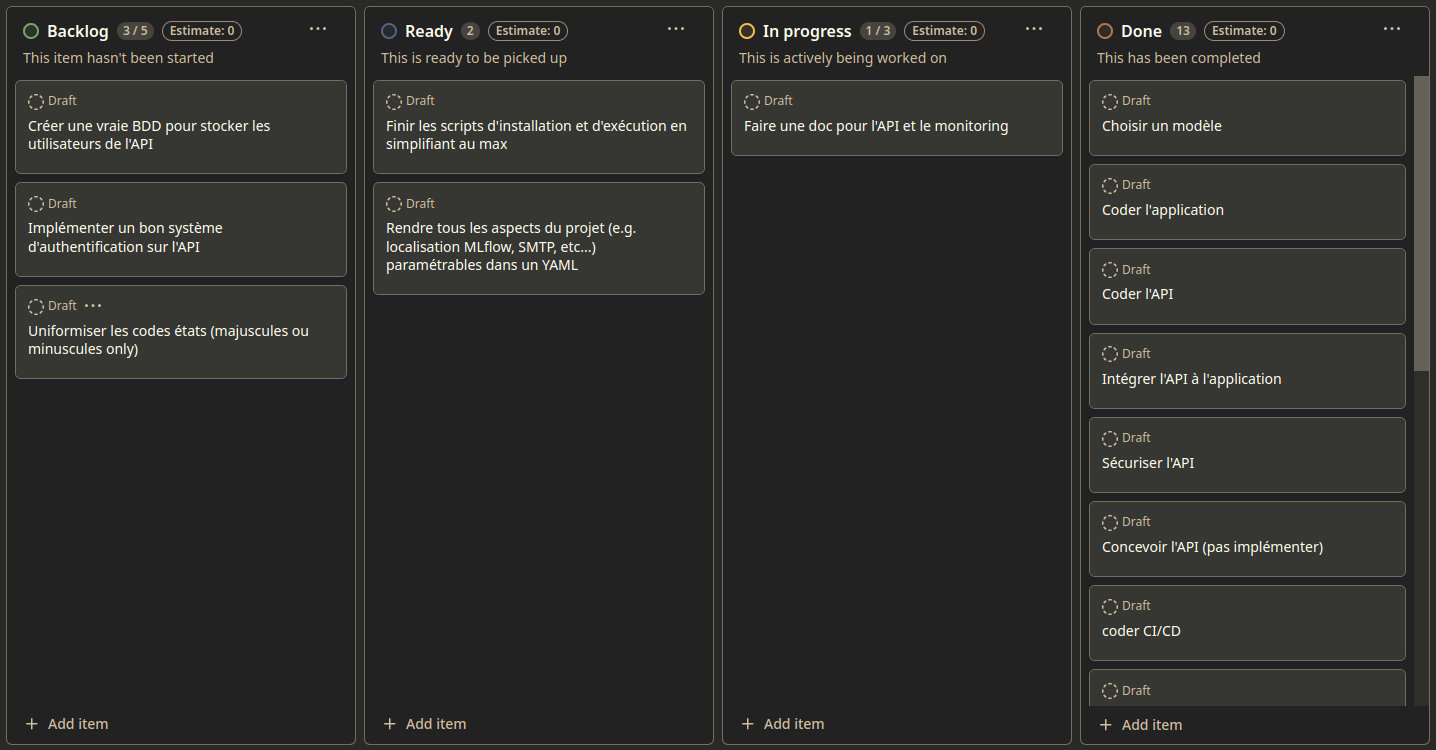
\includegraphics[width=12cm]{kanban}
        \centering
        \caption{Tableau kanban du projet. On remarque que des limites sont imposées au nombre de tâches non commencées ou en cours.}
        \centering
    \end{figure}

    \section{Architecture générale du projet}
    Le service d'IA est constitué de plusieurs composants :
    \begin{itemize}
        \item un modèle d'intelligence artificielle entraîné avec les données fournies par l'Argus. Il prédit ensuite une estimation de prix en fonction des données entrées par l'utilisateur.
        \item une API qui expose ce modèle. C'est le seul composant qui interagit avec l'application web IArgus. Lorsque l'utilisateur soumet un formulaire avec les informations de son véhicule, celles-ci sont automatiquement transmises de façon sécurisée à l'API via une requête HTTP. L'API communique ensuite avec le modèle pour obtenir une estimation de prix et renvoie le résultat à l'application, qui peut l'afficher pour l'utilisateur. Pour les besoins de ce dossier, nous avons déployé cette API sur \textbf{Microsoft Azure} à l'adresse suivante : \href{https://vincent-iargus.azurewebsites.net/}{https://vincent-iargus.azurewebsites.net/} 
        \item un dashboard qui permet aux techniciens de l'équipe informatique de visualiser l'évolution des performances du modèle et de voir l'historique des entraînements et tests réalisés. Ce dashboard a été déployé localement dans le cadre de ce dossier, mais il est aussi possible de le déployer à l'aide d'outils tels que Microsoft Azure
        \item un script de monitoring. Exécuté une fois par mois pour tenir compte des nouvelles données reçues, il teste le modèle avec les nouvelles données et lance un nouvel entraînement si ses performances se sont trop dégradées (i.e. si l'erreur moyenne du modèle a dépassé 20\%). Dans le cas où l'erreur resterait malgré tout trop élevée après cela, le script envoie une alerte par e-mail à l'équipe technique. Ce script est déployé et automatiquement exécuté sur \href{https://www.pythonanywhere.com/}{PythonAnywhere}
        \item une base de données MySQL qui stocke toutes les données utilisées par le modèle. Les nouvelles données reçues chaque mois par l'Argus y sont automatiquement ajoutées. Pour notre projet, nous avons déployé cette base de données sur Microsoft Azure.
    \end{itemize}

    \begin{figure}[h!]
        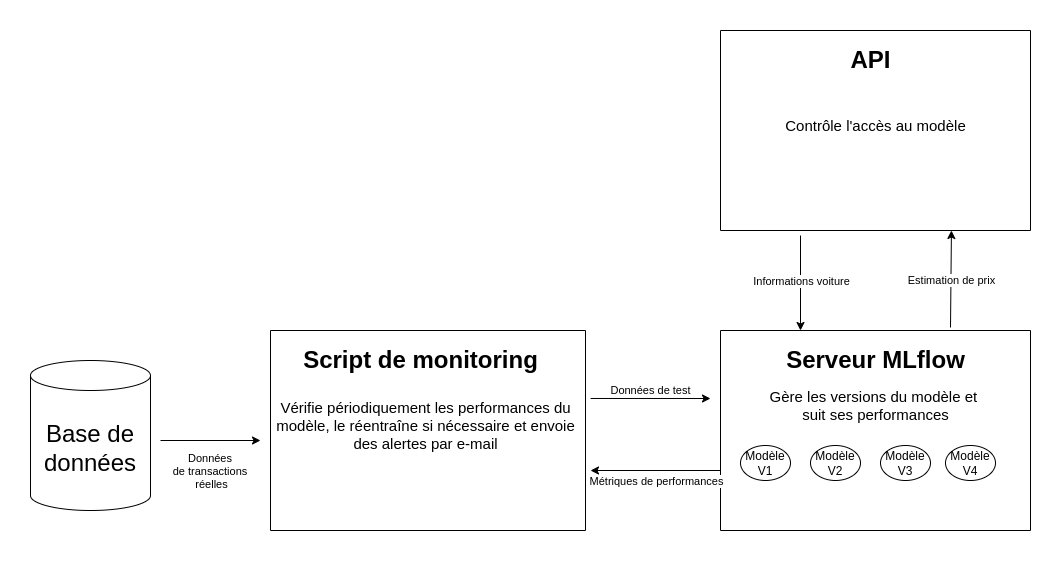
\includegraphics[width=12cm]{architecture_E3}
        \centering
        \caption{Schéma général d'IArgus. Les estimations de prix sont récupérées en passant par l'API qui contrôle l'accès au modèle d'IA.}
        \centering
    \end{figure}

    \section{L'API}
    \subsection{Le modèle d'intelligence artificielle}
    Le modèle d'intelligence artificielle utilisé pour réaliser les estimations de prix est un \textbf{Deep Neural Network} (abrégé DNN), ou \textbf{Réseau Neuronal Profond} en français. Un réseau neuronal est un type de modèle d'intelligence artificielle inspiré par le cerveau humain, plus précisément par les neurones et les connexions synaptiques entre eux. C'est un type de machine learning appelé deep learning qui consiste à utiliser des neurones ou nodes interconnectés, organisés en plusieurs couches. Ce modèle a été choisi suite à la réalisation d'un processus de benchmarking qui a opposé le DNN à plusieurs autres modèles tels que SGD et SVR.

    
    \begin{figure}[h!]
        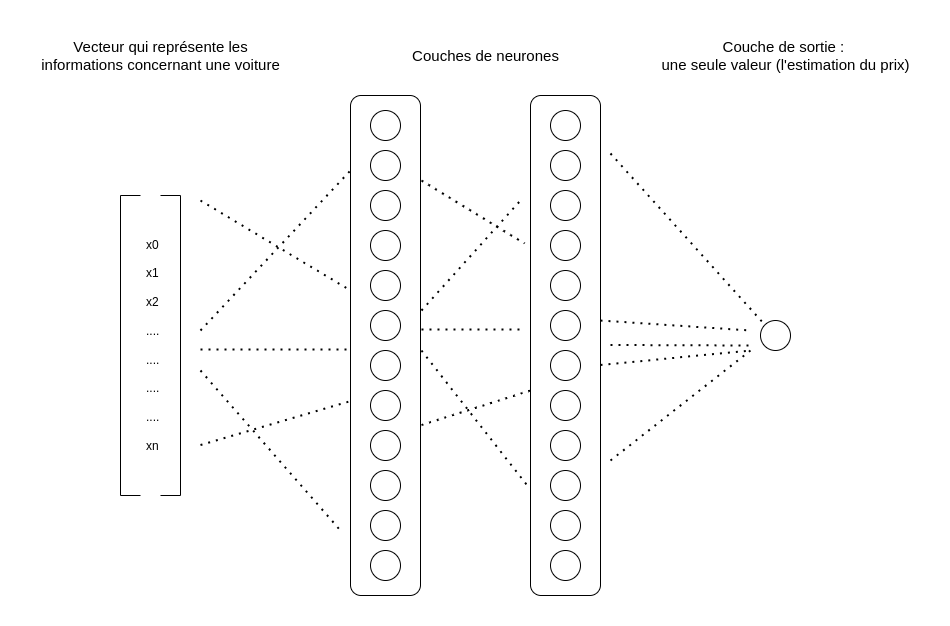
\includegraphics[width=12cm]{dnn}
        \centering
        \caption{Un DNN est composé de couches successives de neurones. Ici, une représentation du réseau utilisé par IArgus : après avoir été numérisées pour constituer un vecteur, les informations concernant la voiture sont traitées par deux couches de neurones avant de passer par une couche de sortie. Cette couche de sortie calcule une unique valeur qui représente le prix estimé par notre modèle.}
    \end{figure}

    Toutes les données disponibles ne sont pas utilisées par le modèle. Parmi les données disponibles pour chaque vente de voiture, seules les informations suivantes sont utilisées :
    \begin{itemize}
        \item le prix de vente
        \item l'année de production de la voiture
        \item le nombre de kilomètres qu'elle a parcourus
        \item l'état américain où la vente a eu lieu
        \item la marque de la voiture
        \item son modèle.
    \end{itemize}
    Le VIN n'est pas utilisé car il s'agit d'un identifiant purement administratif destiné à assurer le suivi d'un véhicule. Il est créé à partir d'informations telles que la ville de production de la voiture, un code de sécurité, et le numéro de série de la voiture, entre autres données. Les informations pertinentes incluses dans ce numéro comme la marque de la voiture étant déjà disponibles dans notre jeu de données, nous n'utiliserons donc pas le VIN ici.
    La ville où se déroule la vente de voiture n'est pas non plus utilisée par notre modèle. Dans ce cas, ce choix est fait dans un souci de performances. En effet, un DNN ne peut traiter que des données numériques : les informations telles que la marque de la voiture, son modèle, la ville ou l'état de la transaction doivent être \textbf{encodées} pour être exploitables par le modèle d'IA. Ceci est accompli grâce à la technique du \textbf{One-Hot Encoding}, qui consiste à convertir des valeurs discrètes (un nom de marque, par exemple) en vecteurs constitués de 1 et de 0 uniquement. Or, la taille de ce vecteur dépend du nombre de valeurs uniques présentes dans nos données pour chaque variable (56 dans le cas de l'état, par exemple). Utiliser cette technique pour convertir le nom de la ville en nombres génèrerait des vecteurs à plusieurs milliers de dimensions, ce qui augmenterait considérablement les besoins en terme de mémoire vive et de puissance de calcul. Toutes ces raisons expliquent pourquoi la ville de vente a été mise de côté.
    
    Une fois que notre DNN est entraîné avec les données fournies par l'Argus, il devient possible de l'utiliser pour estimer des prix de vente. Cependant, l'application n'interagit pas directement avec le modèle. À la place elle envoie des requêtes à un composant qui fait office d'intermédiaire, \textbf{l'API}.


    \subsection{Implémentation de l'API}

    \textbf{Remarque} : l'API présentée ici est implémentée dans le fichier \href{https://github.com/vinpap/iargus/blob/08493c829a37590847164a2f695db763736b9e35/iargus/api.py}{api.py}, dans le dossier iargus du dépôt.

    L'accès au modèle est contrôlé par une API (\textbf{Application Programming Interface}). Une API sert de façade à un ensemble de fonctionnalités : elle permet à un tiers d'utiliser ces fonctionnalités sans avoir besoin de connaître leur fonctionnement interne. Dans notre cas, notre API permet à des tiers (l'application IArgus, les techniciens de l'équipe de développement) d'utiliser notre modèle d'IA sans connaître les rouages de son fonctionnement.

    Utiliser une API pour donner accès à un service confère plusieurs avantages :
    \begin{itemize}
        \item offrir une fonctionnalité via une API permet de contrôler qui accède à notre service, et de quelle manière. En ce qui concerne IArgus, des système d'authentification, de cryptage des communications et de validation des données fournies sont mis en place
        \item les API web telles que celle utilisée dans ce projet permettent de standardiser les communications avec l'API. Dans la mesure où toutes les requêtes à l'API sont réalisées selon le protocole HTTPS, il devient possible d'intégrer rapidement les fonctionnalités de l'API à d'autres projets en cas de besoin
        \item il existe plusieurs outils et frameworks qui permettent de mettre en place rapidement des API. 
    \end{itemize}
    Une API web accepte des requêtes via plusieurs \textbf{endpoints} ("points de terminaison" en français). Chaque endpoint peut accepter une ou plusieurs méthodes de requêtes HTTPS. Voici les points de terminaison utilisés par l'API d'IArgus :
    \begin{itemize}
        \item / (racine de l'API) : ce endpoint renvoie un message d'aide qui explique comment utiliser l'API. Il accepte la méthode GET
        \item /predict : permet de demander à l'IA une estimation de prix à partir des informations envoyées avec la requête. Ce endpoint accepte les requêtes POST.
        \item /get\_token : ce endpoint permet à un utilisateur d'obtenir un token de sécurité qui lui permettra d'utiliser l'API. Ce mécanisme de sécurité est présenté juste après.
    \end{itemize}

    \begin{figure}[h!]
        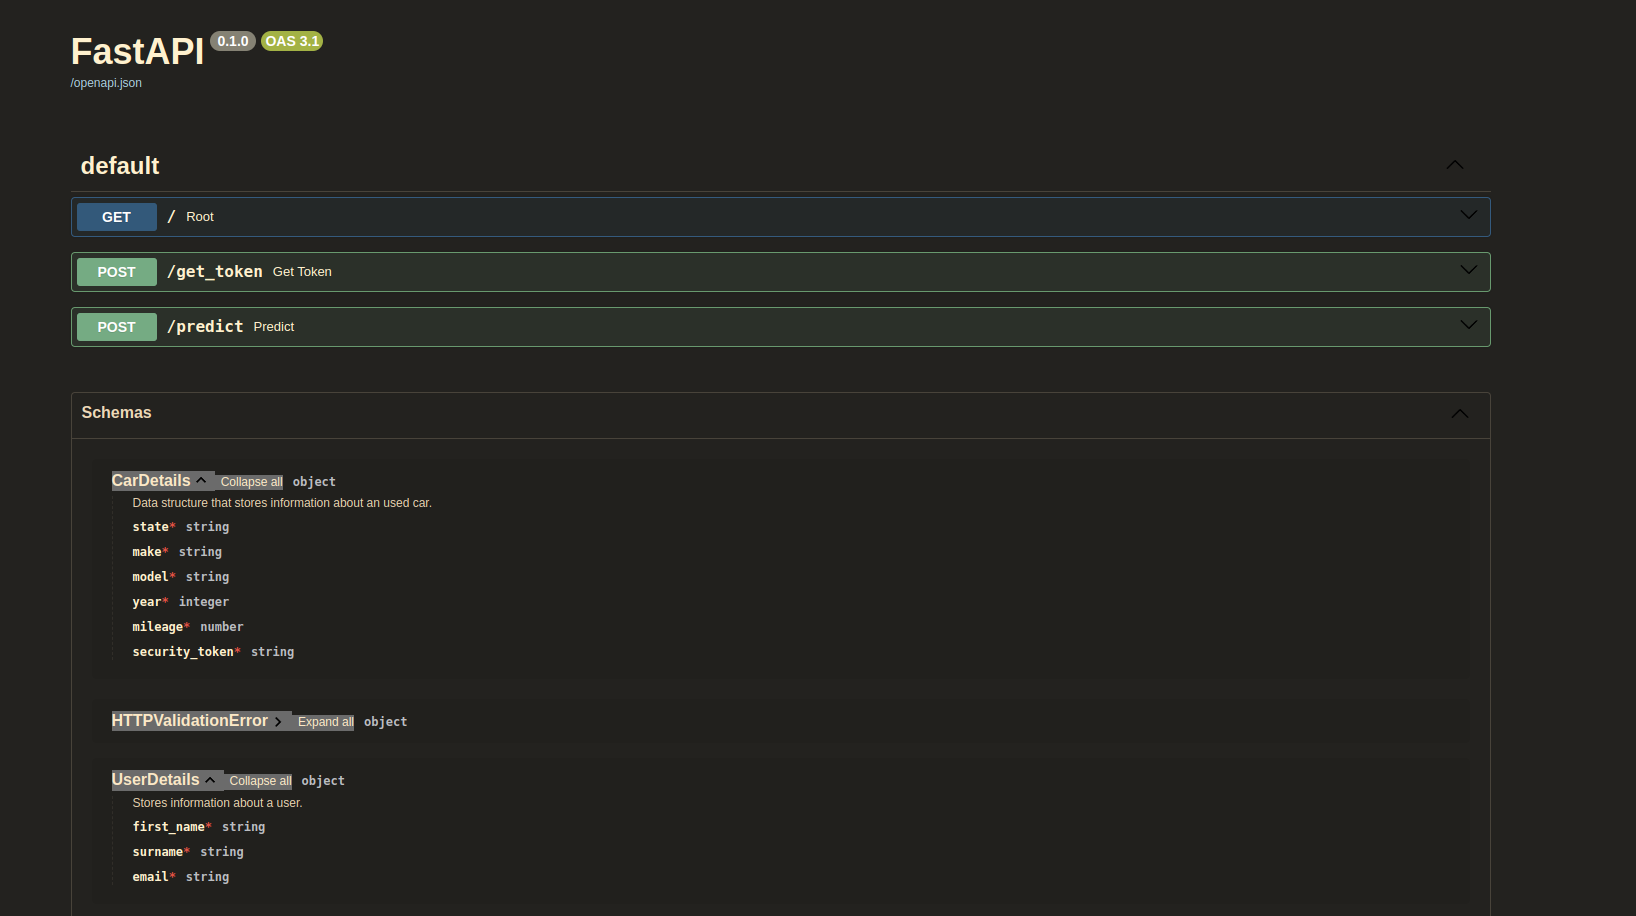
\includegraphics[width=12cm]{api_endpoints}
        \centering
        \caption{Liste des endpoints implémentés dans notre API avec les méthodes HTTP qu'ils acceptent. Les schémas de données "CarDetails" et "UserDetails" présentés en bas de la page détaillent les données qui doivent être envoyées avec les requêtes à /predict et /get\_token, respectivement}
        \centering
    \end{figure}
    Afin de répondre aux exigences du client concernant la sécurisation de l'accès au modèle, plusieurs mécanismes de sécurité ont été implémentés pour réguler l'accès au modèle et protéger l'API des cyberattaques. 
    
    Le premier de ces mécanismes est la création d'un mécanisme d'authentification via un token secret propre à chaque utilisateur. Pour pouvoir utiliser l'API, un utilisateur doit préalablement obtenir un token secret généré aléatoirement. Ce token est généré en envoyant une requête POST au endpoint /get\_token, et doit ensuite être envoyé avec chaque requête aux endpoints / et /predict. \textbf{Le token obtenu n'est valide que pendant 180 jours}. Passé ce délai, l'utilisateur devra en demander un nouveau.

    \begin{figure}[h!]
        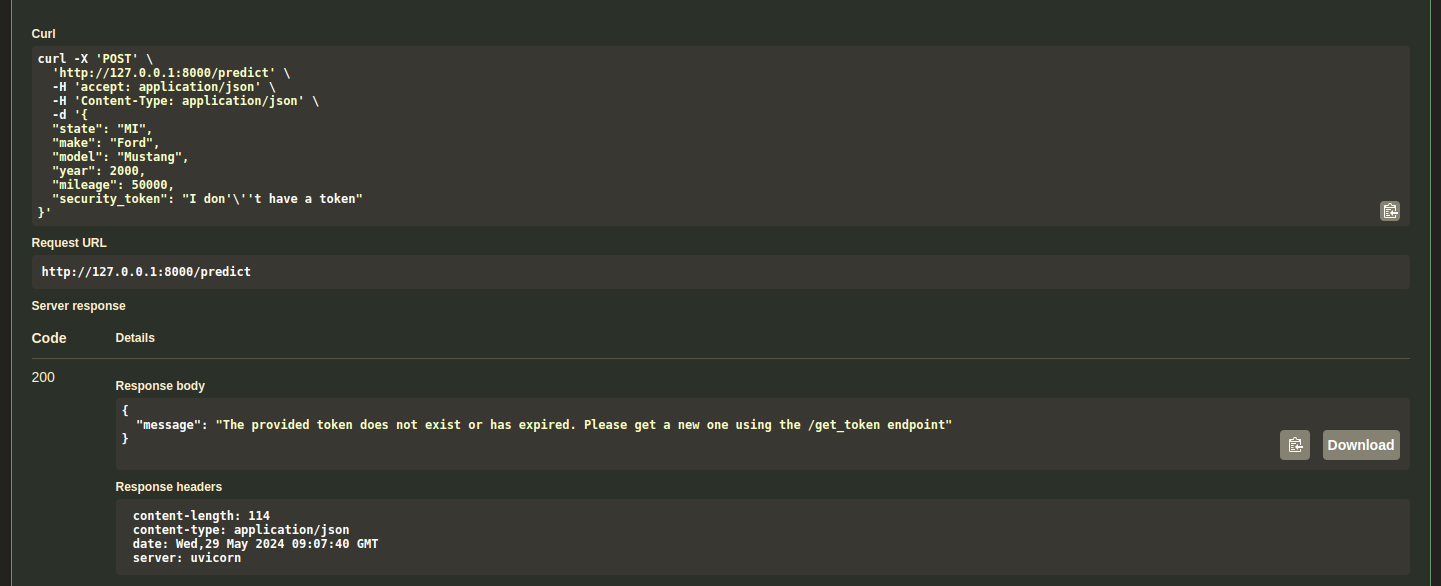
\includegraphics[width=12cm]{api_1}
        \centering
        \caption{Exemple de requête envoyée sans token valide à /predict. Le endpoint renvoit un message d'erreur dans ce cas-là}
        \centering
    \end{figure}

    Pour pouvoir obtenir un token, l'utilisateur doit envoyer avec sa requête à /get\_token son nom, son prénom ainsi que son adresse e-mail. Ces informations sont insérées dans une base de données MySQL avec le token généré ainsi que sa date de création. Cette date est utilisée pour vérifier qu'un token n'a pas expiré.

    \begin{figure}[h!]
        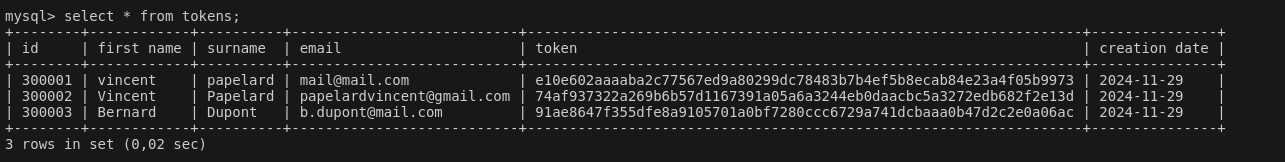
\includegraphics[width=12cm]{db_tokens}
        \centering
        \caption{Les tokens sont stockés dans la table "tokens" d'une base de données MySQL}
        \centering
    \end{figure}

    Les requêtes sans clé valide sont refusées par l'API, ce qui permet d'éviter que des utilisateurs extérieurs à l'entreprise ou des pirates informatiques n'utilisent l'API sans permission.

    Il est important de mentionner que cette mesure \textbf{ne suffit pas, à elle seule, à empêcher des personnes non autorisées à accéder à l'API.} En effet, n'importe qui peut accéder au endpoint /get\_token. Cependant, le token qui a été envoyé avec une requête peut permettre d'identifier la personne à l'origine de cette requête, ce qui peut notamment être intéressant dans une organisation. Pour véritablement empêcher des personnes non autorisées à accéder à l'API, une solution est de \textbf{tenir une "whitelist" d'adresses IP autorisées à faire des requêtes à l'API}. C'est une solution mise en place dans le cadre de ce projet qui sera détaillée dans la section \ref{mise_en_place}.


    Un autre mécanisme de sécurité implémenté est la limitation du nombre de requêtes qu'un utilisateur peut envoyer à l'API dans un court laps de temps. Cela nous permet de protéger notre système des attaques par déni de service, qui consistent à effectuer un grand nombre de requêtes à une URL en un temps très court afin de submerger les capacités du serveur et de le rendre hors service. Dans notre cas, cette protection est d'autant plus importante que notre modèle d'IA consomme beaucoup de mémoire et de ressources de calcul. Ainsi, un grand nombre de requêtes simultanées à /predict pourrait rapidement submerger le serveur où notre IA est déployée.

    Notre API utilise également le protocole \textbf{HTTPS} pour plus de sécurité. Cette extension du protocole HTTP permet de crypter les données qui circulent entre le serveur où se trouve l'API et les clients. Ainsi, il devient impossible pour un pirate informatique d'espionner les données qui circulent entre l'application IArgus et l'API (comme des clés d'API secrètes, par exemple).

    Enfin, notre API réalise une validation des données qu'elle reçoit. Autrement dit, des mécanismes ont été mis en place pour s'assurer que les informations envoyées par l'utilisateur sont bien conformes à ce qui est attendu. Pour le endpoint /predict, par exemple, cela consiste à s'assurer que le nom de l'état est bien une chaîne de caractères, l'année un entier, etc... Ceci nous permet de nous assurer qu'un utilisateur distrait ou mal intentionné ne peut pas faire bugger notre système en envoyant le mauvais type de données.

    L'API a été développée en Python avec le framework FastAPI. FastAPI est conçu pour développer rapidement des API web performantes. De plus, FastAPI offre des fonctionnalités qui permettent de rapidement mettre en place des mécanismes tels que la limitation du nombre de requêtes ou la validation des données entrantes.

    \subsection{Intégration à l'application existante}

    \begin{figure}[h!]
        
\includegraphics[width=12cm]{prediction_result}
        \centering
        \caption{Une page web a été ajoutée à l'application IArgus pour communiquer l'estimation de prix à l'utilisateur.}
    \end{figure}

    Il nous reste maintenant à intégrer l'API d'IArgus à l'application web existante. Comme nous l'avons mentionné dans la section qui décrit le fonctionnement de l'API, un avantage des API est qu'elles permettent d'intégrer facilement une fonctionnalité à une application. Dans notre cas, l'intégration a été réalisée en modifiant la fonction Python qui gère la façon dont les requêtes envoyées à l'URL de la page du formulaire sont traitées. Lorsqu'un formulaire est soumis, l'application envoie une requête à l'URL où est déployée l'API IArgus avec les informations entrées par l'utilisateur (pour plus de flexibilité, l'URL de l'API est définie dans un fichier YAML facilement modifiable). Une fois la prédiction réalisée et le prix estimé renvoyé par l'API, l'application affiche une page web qui montre le prix à l'utilisateur.

    Le token de l'API est stocké dans une variable d'environnement sur le serveur qui exécute l'application. Cependant, il faut également prévoir les cas suivants :
    \begin{itemize}
        \item aucun token n'est défini
        \item un token est défini, mais il a expiré.
    \end{itemize}

    Lorsqu'un utilisateur valide le formulaire avec les informations de sa voiture, une vérification est effectuée pour vérifier ces deux conditions. Si l'application n'a effectivement pas de token valide, elle envoit alors automatiquement une requête au endpoint /get\_token de l'API, en lui donnant pour identifiants les nom, prénom et adresse e-mail de l'administrateur qui sont stockés dans le fichier de configuration de l'application \href{https://github.com/vinpap/iargus_app/blob/386366798c97bc3b68ac874ca10d640cb5d20902/config.yml}{config.yml}. Le token renvoyé par l'API est alors stocké en variable d'environnement, et une nouvelle requête est envoyée à /predict, cette fois-ci avec le nouveau token.

    \section{Monitorage du modèle}

    Le suivi du modèle englobe les composants qui nous permettent de visualiser les performances du modèle au cours du temps et d'envoyer des alertes si jamais celles-ci passent en-dessous d'un seuil acceptable. 
    
    Avant de détailler le fonctionnement de ces composants, parlons de la métrique utilisée pour évaluer les performances de notre modèle. Lors de la présentation des exigences du client, nous avons vu que ce dernier souhaitait garantir que les prix prédits se situaient en moyenne dans un intervalle de 20\% autour des prix réels. Ce critère de performances correspond à \textbf{l'erreur absolue moyenne en pourcentage}, souvent appelée \textbf{MAPE} pour "Mean Absolute Percentage Error". Cette métrique nous indique le pourcentage moyen d'erreur d'un modèle par rapport aux valeurs réelles, ce qui correspond bien à ce que nous demande notre client. Par conséquent, \textbf{la MAPE sera utilisée comme métrique de référence dans la suite de ce dossier.} On considèrera ainsi qu'une MAPE de 20\% resprésente le seuil de performances à ne pas dépasser. Un modèle qui a une MAPE supérieure à ce seuil devra donc être \textbf{réentraîné}.

    \begin{figure}[h!]
        \begin{equation}MAPE = \frac {\sum \frac{\lvert A-P \rvert}{A} \times 100}{N}  \end{equation}
        \centering
        \caption{Définition de la MAPE. Ici $N$ représente le nombre total de prédictions réalisées, $A$ est la valeur réelle du prix, et $P$ la valeur prédite par le modèle d'IA}
        \centering
    \end{figure}

    Le monitorage du modèle est assuré par trois composants de notre projet :
    \begin{itemize}
        \item un script de monitorage exécuté automatiquement à intervalles réguliers qui teste le modèle, le réentraîne si besoin et envoie des alertes par e-mail en cas de problème
        \item un dashboard généré par MLflow, hébergé sur un serveur local
        \item la base de données MySQL qui contient toutes les informations concernant les ventes de voitures d'occasion, continuellement alimentée par l'Argus.
    \end{itemize}

    \subsection{Le script de monitorage}

    Le script de monitorage est \href{https://github.com/vinpap/iargus/blob/981ff9fa80fa4b729df37a93b5966d41e86d6966/iargus/model_monitoring.py}{model\_monitoring.py}. Dans le cadre de ce dossier, il a été déployé sur \href{https://www.pythonanywhere.com/}{PythonAnywhere} où il est exécuté périodiquement.

    Lors de son exécution, le script de monitorage commence par collecter les données depuis la base de données MySQL. Celles-ci sont stockées dans une table car\_details qui recense également la date d'ajout de chaque transaction dans la base de données. Cette information est essentielle car c'est elle qui permet au script de savoir quelles données utiliser pour tester le modèle. En effet, seules les données ajoutées à la base de données après le dernier entraînement du modèle sont utilisées. L'intérêt est de vérifier que le modèle reste performant même avec des données qu'il n'a jamais vues et d'éviter le \textbf{concept drift}. Le concept drift est un phénomène de dégradation des performances d'un modèle lorsque la relation entre les variables d'entrée et de sortie d'un modèle a changé depuis que celui-ci a été entraîné. 
    
    Nous pouvons donner un exemple concret applicable à notre cas : imaginons qu'une ou plusieurs marques de voiture présentes dans le jeu de données d'entraînement aient subi des crises après l'entraînement du modèle (accidents graves impliquant leurs véhicules, scandales, chute de la demande dans le secteur automobile...). Ces événements sont susceptibles d'influencer les prix de vente des voitures d'occasion. Cependant, notre modèle a été entraîné avant ces événements. Ses prédictions n'en tiennent donc pas compte, et cela peut affecter ses performances. Cet exemple est une illustration du concept drift : \textbf{les relations entre les différentes variables ont changé}.

    

    Dans le cas où la MAPE du modèle serait supérieure à 20\%, le script lance un réentraînement du modèle en utilisant cette fois toutes les données disponibles, anciennes comme nouvelles. Une fois ceci fait, la MAPE du modèle nouvellement réentraîné est calculé. Deux cas de figure sont ensuite possibles :
    \begin{itemize}
        \item la MAPE est repassée sous 20\% et le script termine son exécution
        \item la MAPE reste supérieure au seuil de 20\% malgré le réentraînement du modèle. Dans cette situation, une intervention humaine est nécessaire pour résoudre le problème, et le script va donc automatiquement alerter l'équipe technique d'IArgus.
    \end{itemize}

    \begin{figure}[h!]
        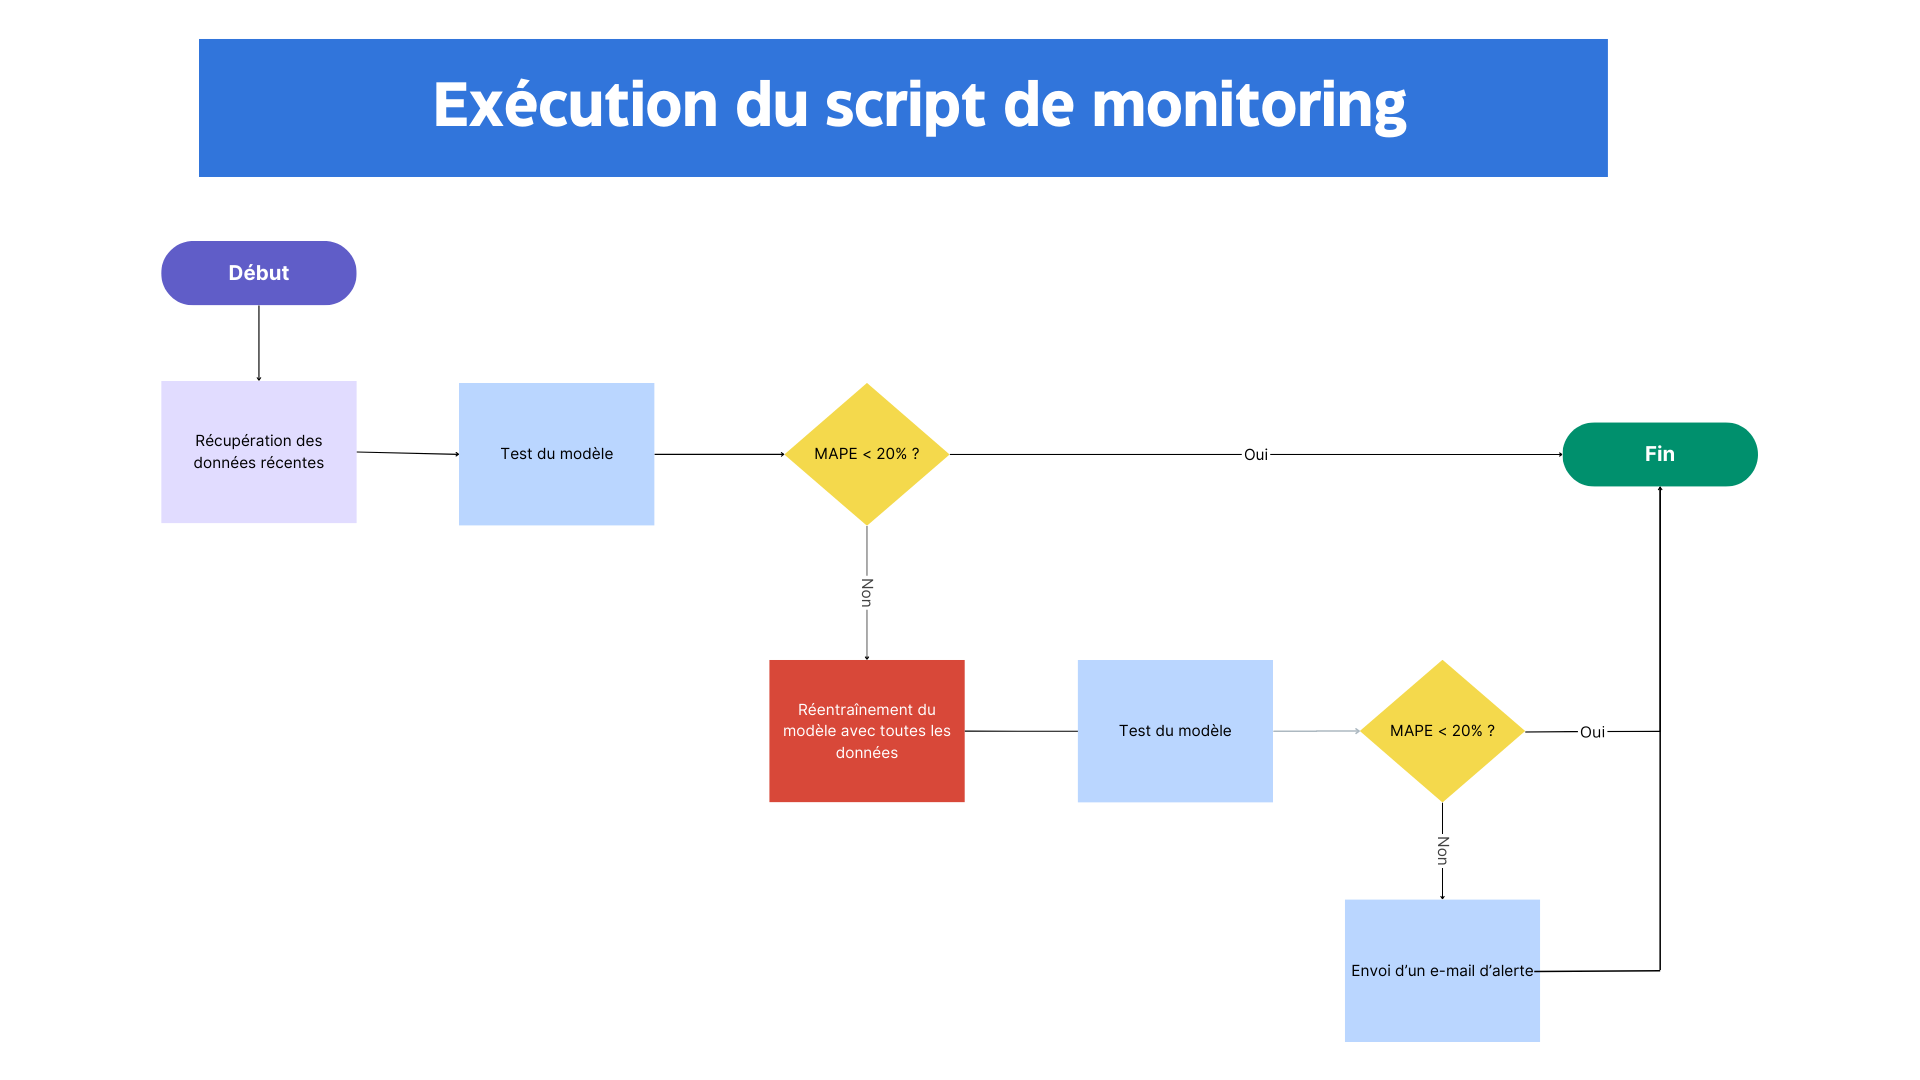
\includegraphics[width=15cm]{monitoring}
        \centering
        \caption{Fonctionnement du script de monitoring.}
    \end{figure}

    \begin{figure}[h!]
        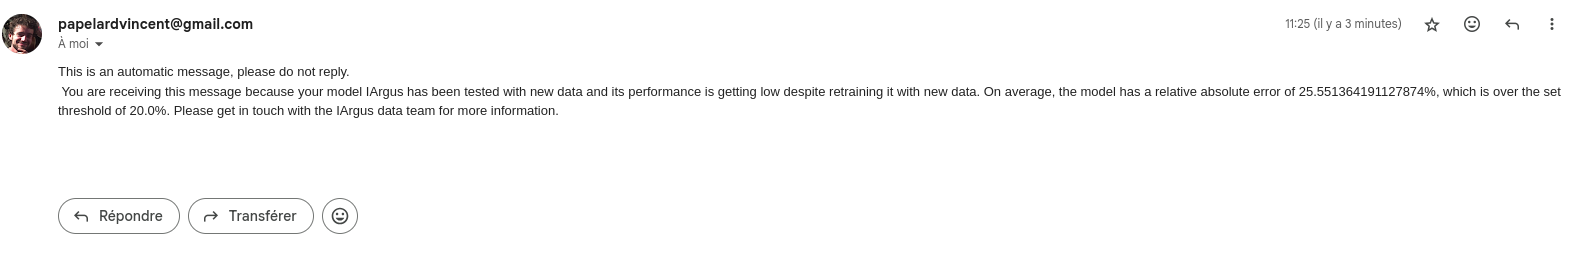
\includegraphics[width=12cm]{mail}
        \centering
        \caption{Un serveur SMTP est nécessaire pour envoyer automatiquement un e-mail. Ici, un exemple d'e-mail envoyé en utilisant le serveur de GMail.}
    \end{figure}

    Dans le deuxième cas, l'alerte est lancée via un e-mail envoyé automatiquement par le script de monitorage. Pour cela, le script passe par un serveur SMTP, dont l'URL et le port à utiliser sont paramétrables dans un fichier de configuration YAML. Il est possible d'utiliser un serveur SMTP comme celui de GMail, ou de coder le sien. Le serveur de GMail a été utilisé pour réaliser les tests nécessaires à l'élaboration de ce dossier.


    \subsection{le dashboard}

    \begin{figure}[h!]
        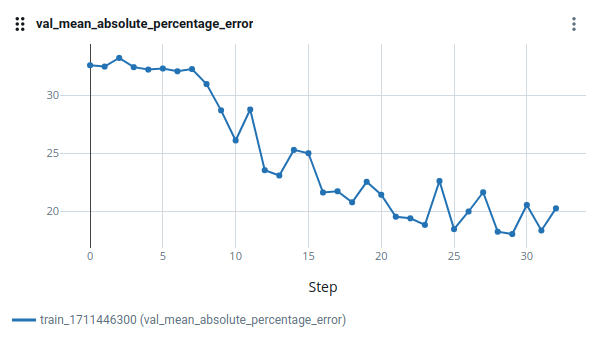
\includegraphics[width=12cm]{mlflow}
        \centering
        \caption{MLflow permet de visualiser les performances du modèle en temps réel. Ce graphique montre l'évolution de la MAPE pendant un entraînement.}
    \end{figure}

    MLflow est utilisé afin de pouvoir suivre le modèle. MLflow permet à l'équipe technique d'IArgus de suivre les performances du modèle dans ses différentes versions, facilitant ainsi la résolution de problèmes de performances éventuels. Le dashboard de MLflow est disponible via un navigateur web et s'exécute en local ou sur un serveur dédié. Nous utilisons MLflow pour notre projet pour sa simplicité d'exécution (une ligne suffit pour lancer un serveur de suivi de modèles) et pour sa facilité d'utilisation (l'interface de Mlflow est très claire et nous permet de trouver facilement les solutions que nous cherchons). Dans la mesure où nous ne savons pas si les techniciens de notre client ont des compétences poussées en intelligence artificielle, il paraît intéressant de leur fournir une interface simple.

    Dans notre cas, nous exécutons MLFlow sur un serveur local rendu public grâce à cette commande :
    \begin{verbatim}
        mlflow server --host <adresse e-mail de la machine qui exécute cette commande>
    \end{verbatim}

    Il est important de noter que le serveur ainsi créé n'est pas sécurisé et reste utilisable par n'importe qui. Deux solutions sont possibles pour pallier à ce problème :
    \begin{itemize}
        \item Définir une liste d'adresses IP autorisées sur la machine où MLflow est exécuté, et refuser les requêtes qui ne proviennent pas de ces adresses IP. Cette solution est cependant très rigide, car il faudrait ajouter une adresse IP à la liste chaque fois qu'un nouvel utilisateur a besoin du serveur MLflow
        \item déployer le serveur MLflow en ligne grâce à un service tel que Databricks ou Azure. Cette approche n'a pas été utilisée ici en raison du coût élevé de ces services, mais il s'agirait d'une bonne solution pour déployer MLflow de manière sécurisée.
    \end{itemize}

    \subsection{La base de données}

    Pour stocker nos données, nous utilisons une base de données MySQL hébergée sur le même serveur que la base de données qui contient les tokens de l'API. Cette base de données contient une seule table, \textit{car\_details}, qui enregistre toutes les ventes de voiture enregistrées aux États-Unis par l'Argus.

    \begin{figure}[h!]
        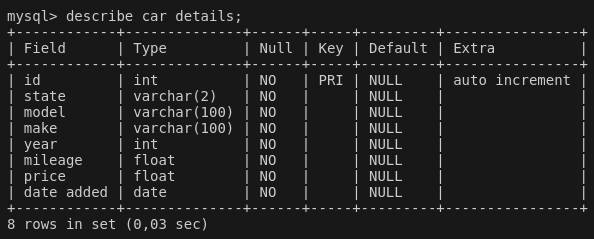
\includegraphics[width=12cm]{car_details_table}
        \centering
        \caption{En plus des différentes informations concernant les voitures vendues, la table car\_details enregistre aussi la date d'ajout de chaque vente, qui est utilisée par le script de monitorage pour savoir quelles données utiliser lors des tests du modèle}
    \end{figure}

    

    \section{Tests et intégration continue}

    Des tests unitaires ont été développés pour garantir le bon fonctionnement d'IArgus. Disponibles dans le dossier \href{https://github.com/vinpap/iargus/tree/08493c829a37590847164a2f695db763736b9e35/iargus/test}{test}, ces tests se divisent en deux catégories :
    \begin{itemize}
        \item les tests unitaires qui vérifient le bon fonctionnement des différentes fonctions du script de monitorage
        \item les tests de points de terminaison codés grâce aux fonctionnalités de test proposées par FastAPI. Ces tests simulent l'envoi de requêtes aux différents points de terminaison de l'API et vérifient que les données renvoyées par l'API sont conformes à celles que l'on attend.
    \end{itemize}

    Les tests du monitorage couvrent les situations suivantes :
    \begin{itemize}
        \item on vérifie que la conversion des variables catégoriques dans les données (comme la marque des voitures, par exemple) a bien fonctionné, notamment en s'assurant qu'une variable encodée en \textit{one-hot} vector ne compte qu'un seul 1 dams le vecteur obtenu
        \item on vérifie également que la MAPE calculée par la fonction de test est bien comprise entre 0 et 1.
    \end{itemize}

    Les tests de l'API couvrent tous les endpoints et vérifient les cas suivants :
    \begin{itemize}
        \item pour la racine / : on vérifie que la requête renvoit un code 422 si on n'a pas envoyé de token
        \item pour /predict : on vérifie que :
        \begin{itemize}
            \item si on n'envoit pas de token avec la requête, aucune prédiction n'est réalisée et on obtient un code d'erreur 422
            \item si on envoit un token valide, une prédiction est réalisée et un float renvoyé
        \end{itemize}
        \item pour /get\_token : on s'assure qu'aucun token n'est renvoyé si l'adresse e-mail fournie ne respecte pas le bon format.
    \end{itemize}

    Par ailleurs, ces tests ont été automatisés grâce à la fonctionnalité \textbf{GitHub Action}. Ainsi, pousser le code local vers le dépôt distant sur GitHub ou fusionner une branche avec la branche master lance automatiquement les tests. Leur exécution est paramétrée dans le fichier de configuration \href{https://github.com/vinpap/iargus/blob/fea8247513304d645d6cb4ff5857fe8951ff95e0/.github/workflows/master_vincent-iargus.yml}{master\_vincent-iargus.yml} lu automatiquement par la machine virtuelle qui exécute les tests sur les serveurs de GitHub. Ce fichier de configuration spécifie une liste de commandes à exécuter dans un ordre précis pour réaliser les actions suivantes :
    \begin{itemize}
        \item installer toutes les dépendances du projet dans un environnement virtuel avec pipenv
        \item lancer MLflow sur l'hôte local
        \item exécuter un script setup\_tests.py qui met en place les différents éléments nécessaires à l'exécution des tests (chargement d'un jeu de données de test fourni dans le dépôt, entraînement d'un modèle avec ces données)
        \item exécuter les tests avec pytest.
    \end{itemize}

    Ces actions sont automatiquement effectuées lorsque du code est poussé ou fusionné sur la branche master (avec une \textit{pull request}).

    \begin{figure}[h!]
        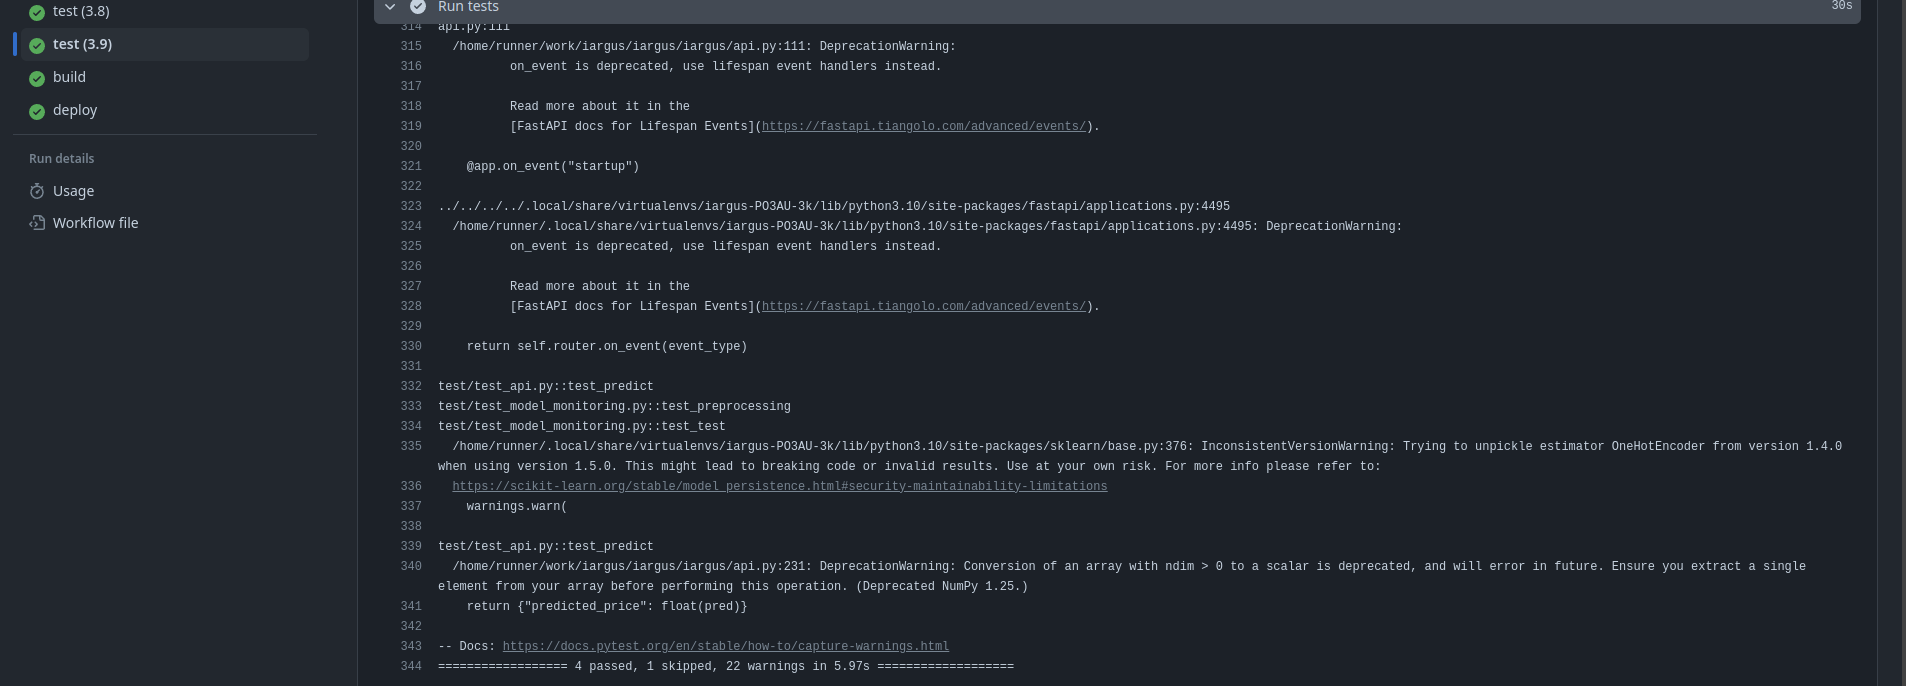
\includegraphics[width=12cm]{gh_action}
        \centering
        \caption{Une capture d'écran de l'interface de GitHub Action. Ici on constate que toutes les étapes de test et de déploiement d'IArgus ont réussi. La ligne en bas de l'écran indique les résultats du test.}
    \end{figure}

    Dans le cas où un ou plusieurs de ces tests échouerait au moment où le code d'IArgus est mis à jour sur GitHub, un e-mail est automatiquement envoyé à l'adresse e-mail de la personne qui a réalisé la mise à jour. Cette fonctionnalité nous permet d'être alerté immédiatement si les dernières modifications apportées au code ont malencontreusement introduit des bugs dans IArgus.


    \section{Livraison continue}
    
    Comme on peut le constater dans la capture d'écran ci-dessus, GitHub Action n'est pas uniquement utile pour l'automatisation de tests. Ici, nous nous en servons également pour déployer automatiquement l'API sur Microsoft Azure. Dans les faits, les actions suivantes sont effectués lorsque du code est poussé ou fusionné sur la branche master :
    \begin{itemize}
        \item comme nous venons de le voir, les tests de l'API et du monitorage sont exécutés
        \item en parallèle, le code est déployé sur Microsoft Azure, qui installe les dépendances nécessaires et lance l'application en utilisant la commande de démarrage spécifiée dans les paramètres de notre application sur la ressource Azure.
    \end{itemize}
    

    \section{Mise en place de IArgus} \label{mise_en_place}

    Cette section couvre la mise en place des différents composants d'IArgus. il s'agit de la documentation présentée dans \href{https://github.com/vinpap/iargus/blob/fca4c4c15cce4cdcf9302b8a4ca29ca033c4686a/README.md}{le fichier README} du dépôt.

    \subsection{Installation de la base de données}
    \subsection{Lancement de MLflow}
    \subsection{Déploiement de l'API}


    \subsection{Mise en place du monitorage}
    \subsection{Intégration de l'API à une application existante}

    \newpage
    \section*{Conclusion}
    
    Ce dossier a présenté l'intégration d'un service d'intelligence artificielle à une application web existante via une API. Toutes les étapes ont été couvertes, du choix du modèle à la conception de scripts d'installation en passant par la mise en place d'un système de tracking des performances de l'IA.

    Cependant, certains aspects du projet restent améliorables :
    \begin{itemize}
        \item pour plus de sécurité, l'API pourrait mettre en place un système de gestion des utilisateurs et générer une clé de sécurité unique pour chacun. Cela éviterait d'utiliser une seule clé de sécurité et permettrait d'authentifier les utilisateurs de l'API
        \item IArgus pourrait être configuré pour envoyer des alertes par e-mail à une liste d'adresses e-mail, et pas à une seule adresse comme c'est le cas actuellement
        \item enfin, des scripts d'installation et d'exécution pourraient être écrits pour permettre de déployer IArgus sur un serveur Windows.
    \end{itemize}

    \addcontentsline{toc}{section}{Conclusion}

    \end{document}